Since Ramon y Cajal discovered that the brain is a rich and dense \emph{network} of neurons \cite{RamonyCajal04,RamonyCajal23}, neuroscientists have been intensely curious about the details of these networks, which are believed to be the biological substrate for memory, cognition, and perception. While we have learned a great deal in the last century about ``macro-circuits'' --- the connectivity between coarsely-defined brain areas --- relatively little is known about ``micro-circuits,'' i.e., the connectivity within populations of neurons at a fine-grained cellular level. Broadly, one can imagine two complementary strategies for inferring microcircuit connectivity: anatomical and functional. Anatomical approaches to inferring circuitry include any strategy that does not consider physiological measurements of neural activity: for example, recently developed technologies including array tomography \cite{MichevaSmith07}, ``brainbow'' mice \cite{Brainbow07}, and serial electron microscopy \cite{Briggman2006} are rapidly improving and show great promise. Our work, on the other hand, takes a functional approach: our aim is to infer microcircuit properties by observing the activity of a population of neurons.

Experimental tools that enable approximately simultaneous observations of the activity of many (e.g., $O(10^3)$) neurons are now widely available. While arrays of extracellular electrodes have been exploited for this purpose, the arrays most often used \emph{in vivo} are inadequate for inferring monosynaptic connectivity, as the inter-electrode spacing is typically too large to record from all of the neurons in a given volume \cite{HATS98,HARR03,Stein04,Santhanam06,Harris07} \footnote{It is worth noting, however, that multielectrode arrays which have been recently developed for use in the retina are capable of much denser sampling \cite{Berry2004,Litke2004,Petrusca07,PILL07}.}. Alternately, calcium-sensitive fluorescent indicators allow us to observe the spiking activity of many neighboring neurons \cite{Tsien89}, which are more likely to be connected \cite{Abeles91, Braitenberg1998}. Some organic dyes achieve sufficiently high signal-to-noise ratios (SNR) that individual action potentials (spikes) may be resolved \cite{ImagingManual}, and bulk-loading techniques enable experimentalists to simultaneously fill populations of neurons with such dyes \cite{StosiekKonnerth03}. In addition, genetically encoded calcium indicators are under rapid development in a number of groups, and are approaching SNR levels of nearly single spike accuracy as well \cite{WallaceHasan08}. Microscopy technologies for collecting fluorescence signals are also rapidly developing. Cooled CCDs for wide-field imaging (either epifluorscence or confocal) now achieve a quantum efficiency of $\approx 90 \%$ with frame rates up to $60$ Hz or greater, depending on the width of the field of view \cite{Djurisic04}. For in vivo work, 2-photon laser scanning microscopy can achieve similar frame rates, using acoustic-optical deflectors to focus light at arbitrary locations in three-dimensional space \cite{ReddySaggau05, Iyer06, SalomeBourdieu06, ReddySaggau08}, or using resonant scanners \cite{NguyenParker01}. Together, these experimental tools can provide movies of calcium fluorescence transients for small populations of neurons (e.g., $O(10^2)$), with ``reasonable'' SNR, at imaging frequencies of 30 Hz or greater, in both the in vitro and in vivo settings.

Given these experimental advances in functional neural imaging, our goal is to develop efficient computational and statistical methods to exploit this data for the analysis of neural connectivity. See Fig.~\ref{fig:data_schematic} for a schematic overview. One major challenge is that calcium transients due to action potentials decay about an order of magnitude more slowly than the time course of the underlying neural activity \cite{ImagingManual}. Thus, to properly analyze the functional network connectivity in this setting, we must incorporate methods for effectively deconvolving the observed noisy fluorescence signal to obtain estimates of the underlying spiking rates \cite{YaksiFriedrich06,GreenbergKerr08,Vogelstein2009}. To this end we introduce a coupled Markovian state-space model that relates the observed variables (fluorescence traces from the neurons in the microscope's field of view) to the hidden variables (spike trains and intracellular calcium concentrations of these neurons), as governed by a set of biophysical parameters including the network connectivity matrix. Given this model, we derive a Monte Carlo Expectation Maximization (MCEM) algorithm for approximating the maximum a posteriori estimates of the parameters of interest. Standard Monte Carlo sampling procedures (e.g., Gibbs sampling or sequential Monte Carlo) are inadequate in this setting, due to the high dimensionality and non-linear, non-Gaussian dynamics of the hidden variables in our model; we therefore develop a specialized blockwise-Gibbs approach to overcome these obstacles. This strategy enables us to accurately infer the functional connection matrix from moderately-sized simulated neural populations, under realistic assumptions about the dynamics and observation parameters. We describe our approach below, along with several methods for improving its computational speed and statistical efficiency.


\begin{figure}[t!]
\centering 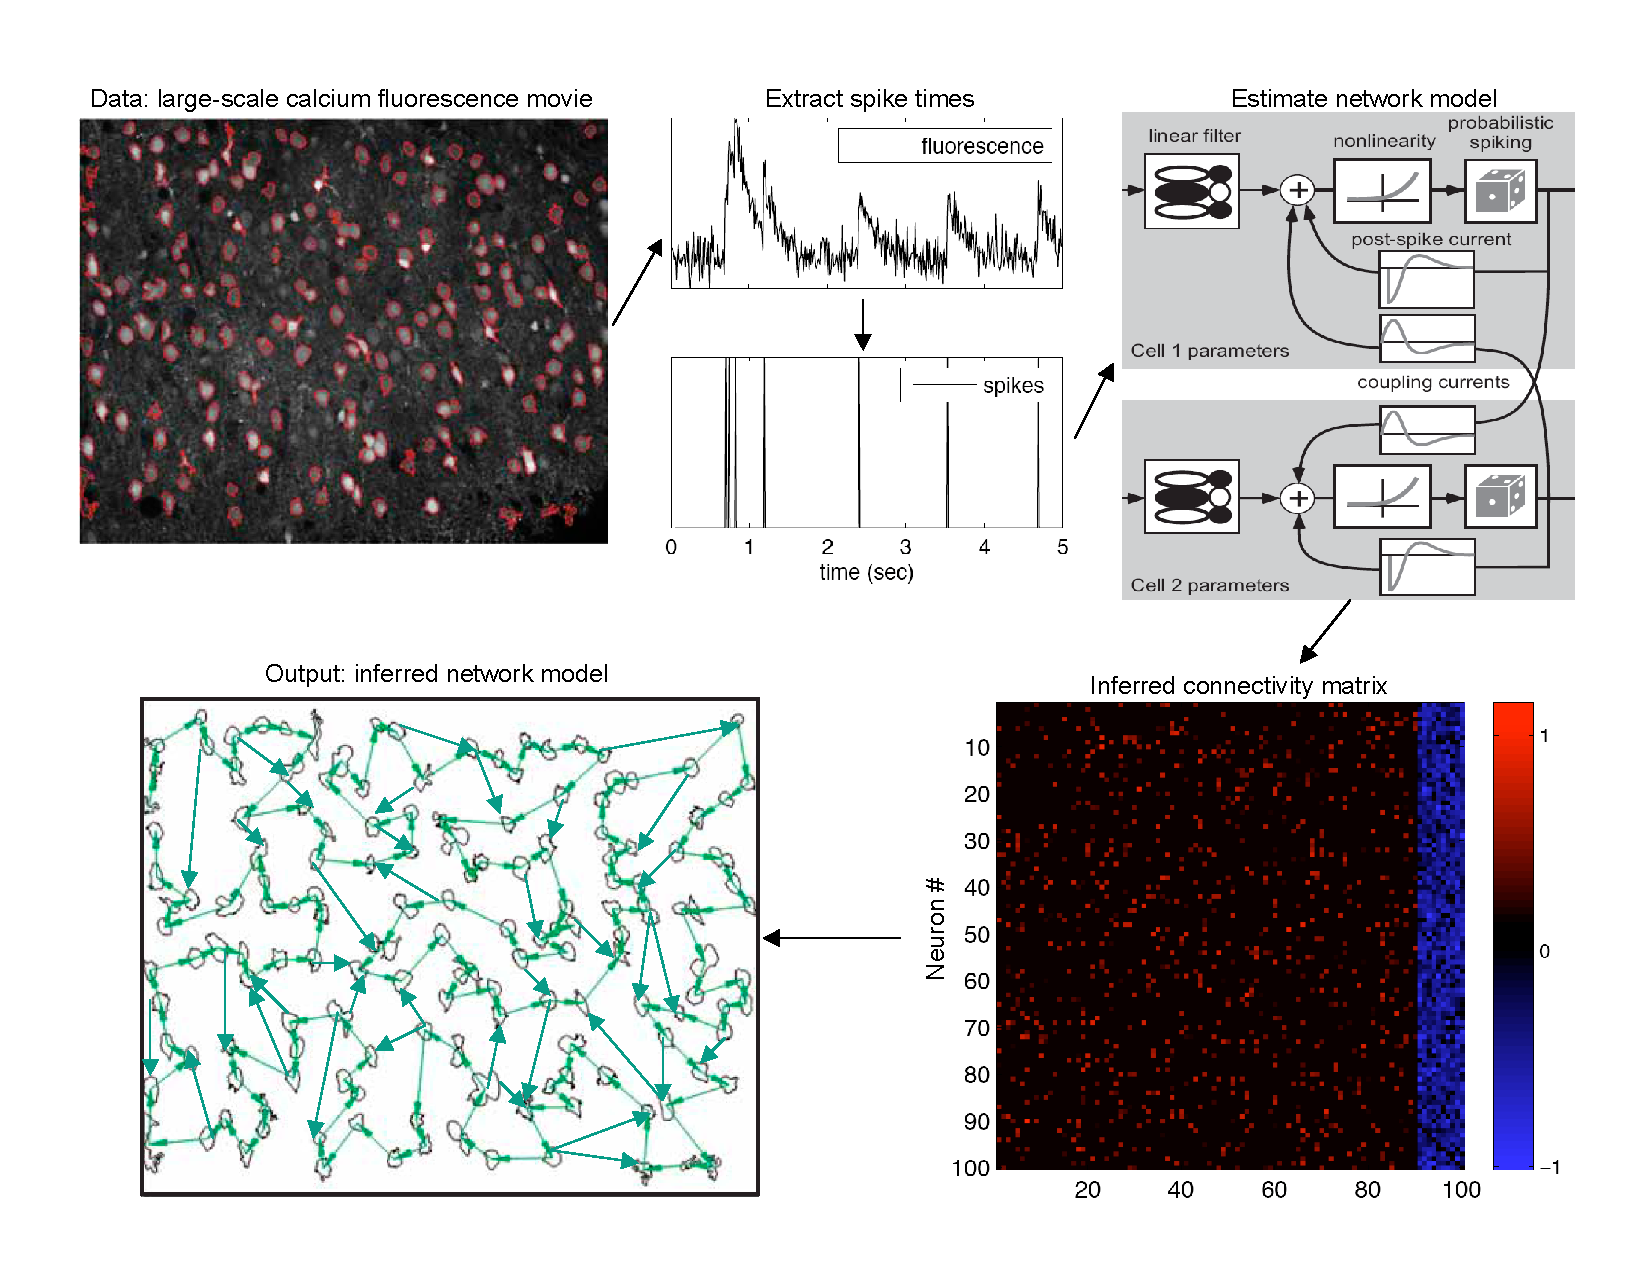
\includegraphics[width=\hsize]{../figs/yuri-paper-schematic}
\caption{Schematic overview. The raw observed data is a large-scale calcium fluorescence movie, which is pre-processed to correct for movement artifacts (in the in vivo setting) and find regions-of-interest (i.e., putative neurons); note that we have omitted details of these important preprocessing steps in this paper. Given the fluorescence traces from each neuron, we estimate the underlying spike trains (i.e., time series of neural activity) using statistical deconvolution methods. Then we estimate the parameters of a network model, given the observed data. Our major goal is to obtain an accurate estimate of the network connectivity matrix, which summarizes the information we are able to infer about the local neuronal microcircuit.}
\label{fig:data_schematic} \end{figure}
